\documentclass[a4paper,11pt]{article}
%
\usepackage{graphicx}
\usepackage{amsmath}
\usepackage{amssymb}
\usepackage{bm}
\usepackage{latexsym}
\usepackage{natbib}
\usepackage{float}
%
\addtolength{\textwidth}{40mm}
\addtolength{\oddsidemargin}{-20mm}
\addtolength{\evensidemargin}{-20mm}
\addtolength{\textheight}{15mm}
\addtolength{\topmargin}{-10mm}
%
\pagestyle{empty}
%
\title{Progress Report}
\author{Simon Sepiol-Duchemin}
\date{\today}
%\date{June 25, 2019}
%
\begin{document}
%
\maketitle
\thispagestyle{empty}
%
\section{Research Objective and Goal}
The objective of this study is to improve the booleanization part of algorithm from \cite{9521203}. Starting with understanding the nonnegative matrix factorization problem and algorithms to solve it.
\section{Short-Term Goals}
\begin{enumerate}
\item Implementing the NFM algorithm presented in \cite{9521203}. Begin to read the paper \cite{9521203}.
\end{enumerate}
\section{Progress}
\begin{enumerate}
\item I have implemented the algorithm using numpy and compared it against the scikit-learn one.
\item I have started reading the paper but have some questions about the update of Y and the regularization. 
\section{Results}
\begin{figure}[H]
    \includegraphics{../../results/distance_results.png}
\end{figure}
\begin{figure}[H]
    \includegraphics{../../results/initial_final_results.png}
\end{figure}
\begin{figure}[H]
    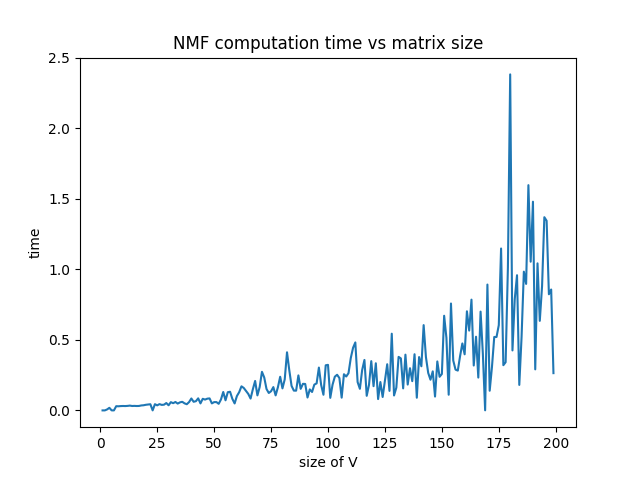
\includegraphics{../../results/time_results.png}
\end{figure}
\end{enumerate}
\bibliographystyle{apalike}

\bibliography{biblio}
\end{document}
